

\section{Background}


The \textit{Global Positioning System} (abbreviated as GPS) is a space-based navigation system consisting of a network of 24 satellites placed in space in six different 12-hour orbital paths \citep{agrawal2015introduction}, so that at least five of them are in view from every point on the globe \citep{kaplan2005understanding, bajaj2002gps}. A GPS device receives signals from these satellites and triangulates its location in terms of longitude, latitude, and elevation. GPS is the most widely known location-sensing system providing an excellent framework for determining geographic positions \citep{hightower2001location}. Offered free of charge and accessible worldwide, GPS has a vast number of applications, including aircraft tracking, vehicle navigation, robot localization, surveying, astronomy, and so on. 

GPS units in vehicles typically record position, speed, and direction of travel. With this information, a target tracking system becomes available and useful. Such a tracking system can be used to reduce costs by knowing in real-time the current location of a vehicle, such as a truck or a bus \citep{chadil2008real}, with applications to  Intelligent Transportation Systems (ITS) \citep{mcdonald2006intelligent}. It can also be used to measure real-time traffic data and to identify congestion areas. In farming applications, a tracking system allows the location and operational status of farm vehicles to be monitored remotely. 


%It is suggested that the smoothing spline fitting through the measured values reflecting the movements is an alternative approach. Even though fitting a univariate local linear trend model using a Kalman filter is equivalent to fitting a cubic spline, see \citep{eubank2004simple, durbin2012time}, the latter algorithm overcomes the current limitation and can approximate data points throughout the whole process. 


Given time series data from a vehicle-mounted GPS unit, an important question is how to infer the trajectory of the vehicle. This is known as trajectory reconstruction and is the motivating question of this thesis. 




\section{The Problem}

Two keys issues for reconstruction are (\romannum{1}) how to handle observations that are inherently noisy measurements of the truth, and (\romannum{2}) how to interpolate appropriately between observation times.

GPS units in vehicles provide $y_t$, noisy measurements of the actual position $x_t$, and $v_t$, noisy measurements of the actual velocity $u_t$, for a sequence of times $t\in T$. These data may also be augmented with information on operating characteristics of the vehicle, $b_t$. The trajectory reconstruction problem is the problem of estimating $x_s$, for an arbitrary time $s$, given a subset of the observations $\{y_t,v_t,b_t\mid t\in T\}$. Note that in this definition of trajectory reconstruction, we are not explicitly interested in estimating $u_s$.


The \textit{TracMap} company, located in New Zealand and USA, produces GPS display units to aid precision farming in agriculture, horticulture and viticulture. Operational data is collected and sent by these units to a remote server for further analysis. An example of position data, which has been subsampled at irregular time points, is given in Figure \ref{tracoverview}. 

%Generally, this data is irregularly sampled every 1 to 30 seconds over the whole day. 
\begin{figure}[h]
	\centering
	\begin{tikzpicture}
	\node[anchor=south west,inner sep=0] (image) at (0,0) {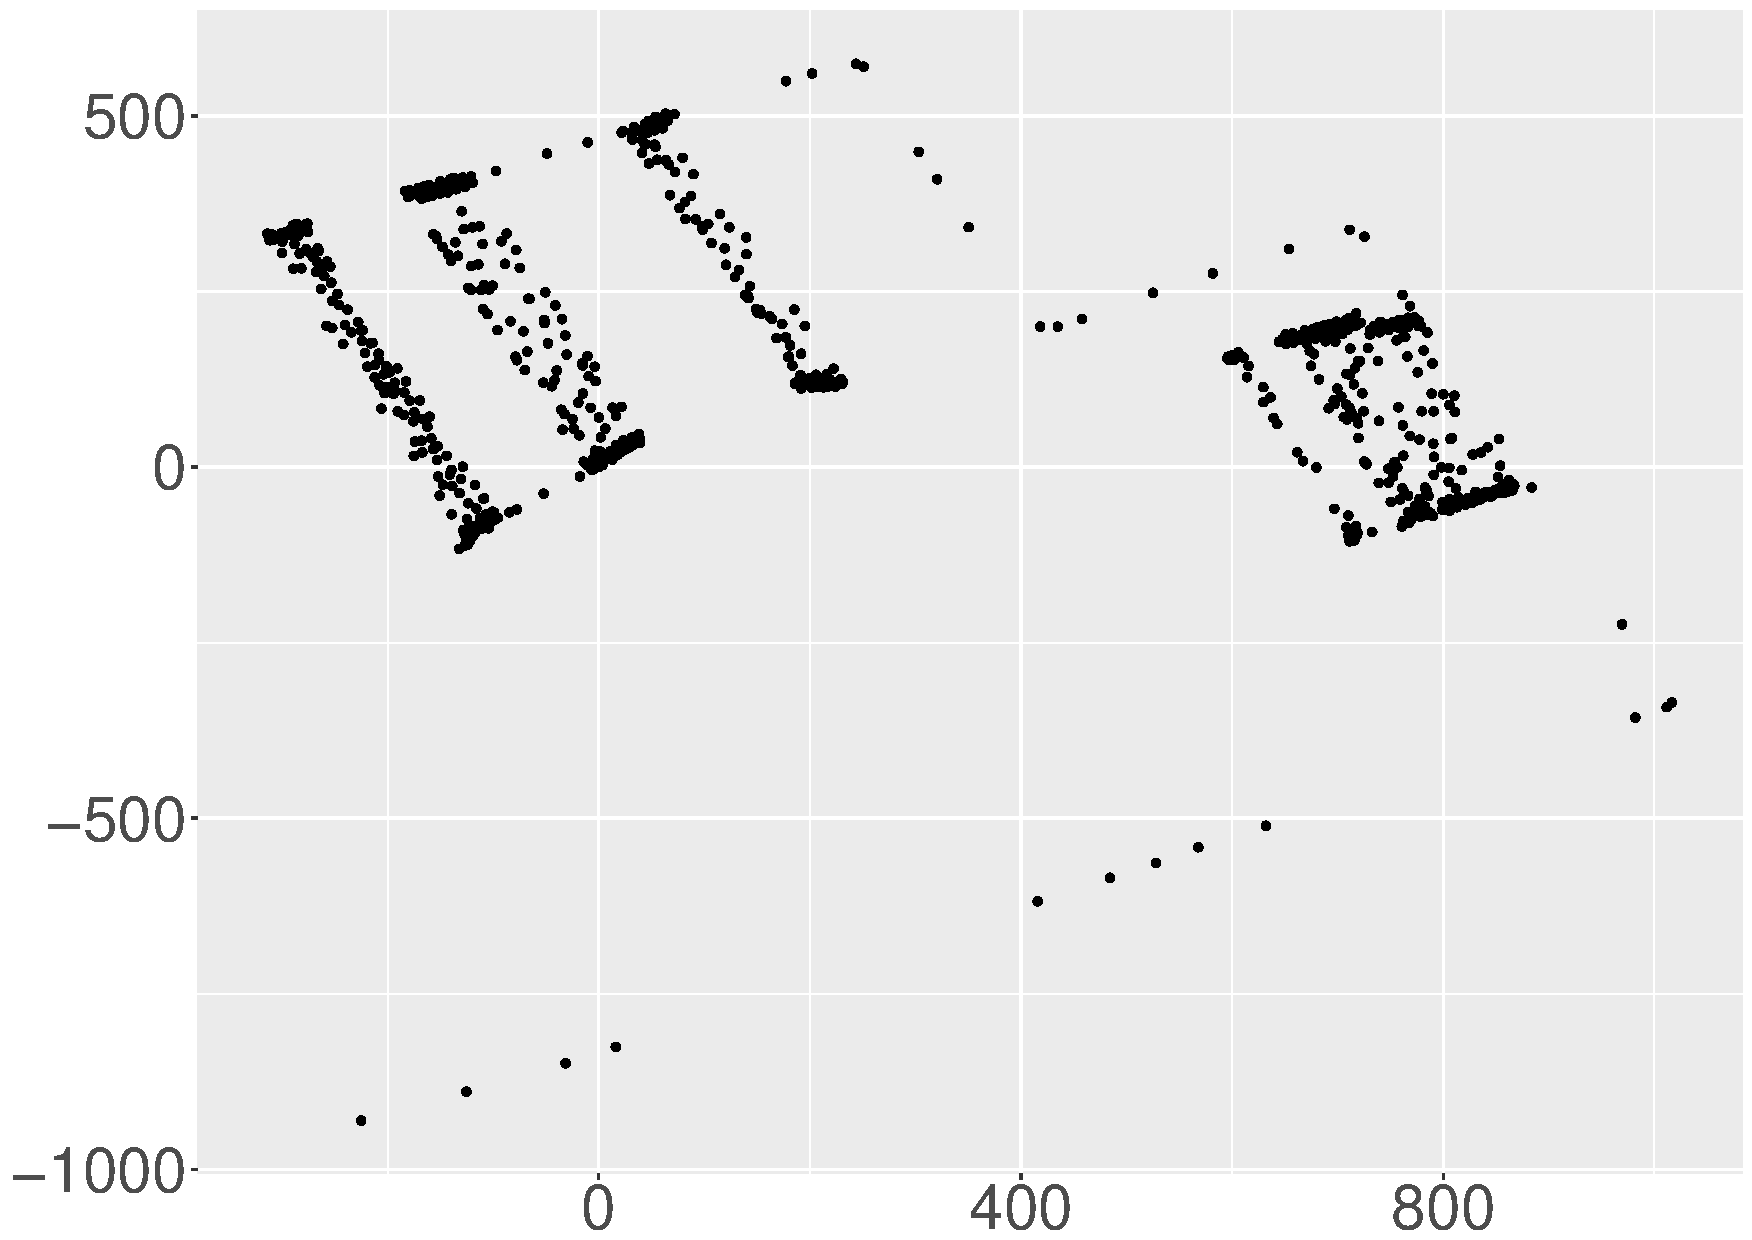
\includegraphics[width=0.45\textwidth]{Chapters/01Intro/plots/tracoverview01.pdf}};
	\begin{scope}[
	x={(image.south east)},
	y={(image.north west)}
	]
	\node [black, font=\bfseries] at (0.5,-0.05) {Easting};
	\node [black, font=\bfseries,rotate=90] at (0,0.5) {Northing};
	\end{scope}
	\end{tikzpicture}
	\begin{tikzpicture}
	\node[anchor=south west,inner sep=0] (image) at (0,0) {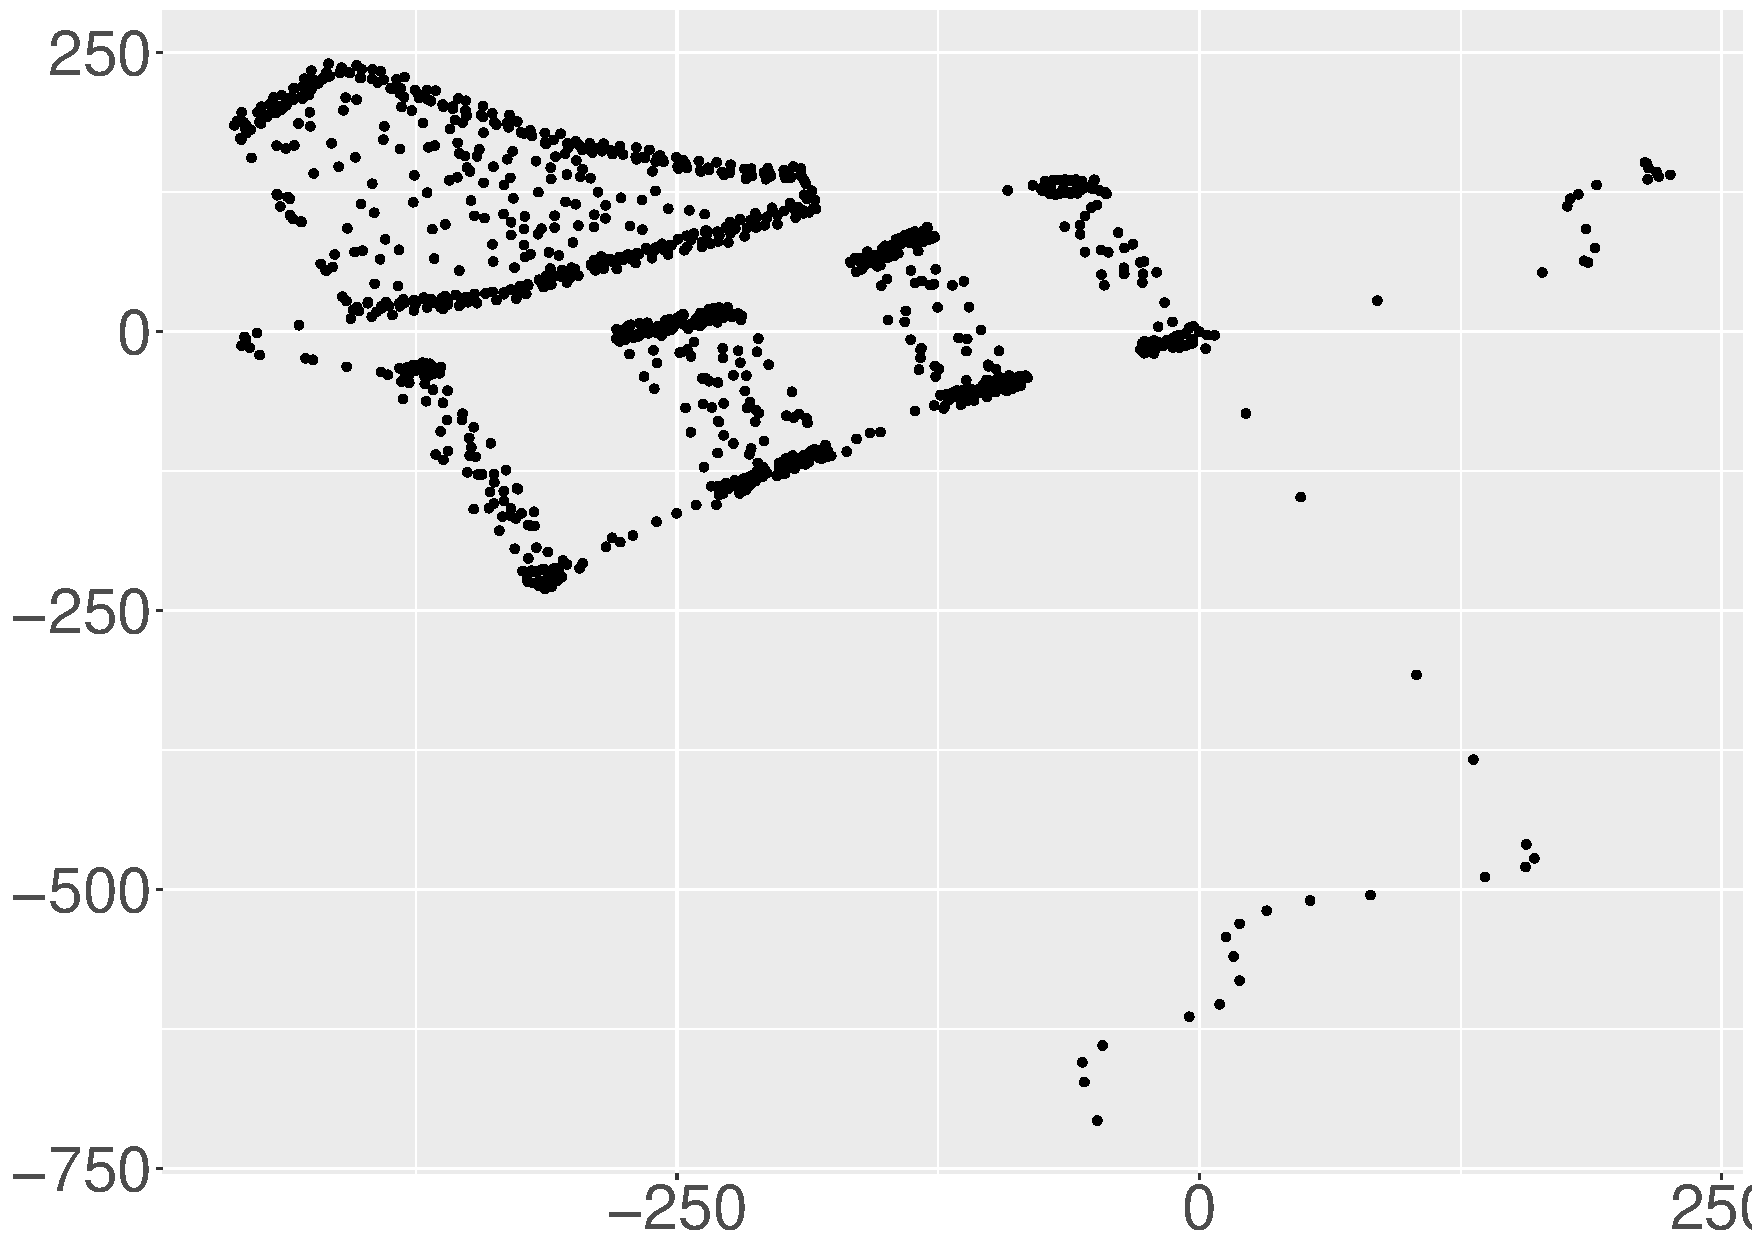
\includegraphics[width=0.45\textwidth]{Chapters/01Intro/plots/tracoverview02.pdf}};
	\begin{scope}[
	x={(image.south east)},
	y={(image.north west)}
	]
	\node [black, font=\bfseries] at (0.5,-0.05) {Easting};
	\node [black, font=\bfseries,rotate=90] at (0,0.5) {Northing};
	\end{scope}
	\end{tikzpicture}
	\caption{Examples of GPS data. Observed positions $y_t$ are shown. In trajectory reconstruction, the $y_t$ are combined with velocity information $v_t$ and operating characteristics $b_t$ to infer actual positions $x_s$, for times of interest $s$.}\label{realGPSdataset}
	\label{tracoverview}
\end{figure}





\section{Smoothing Spline Based Reconstruction}

Smoothing spline approaches are natural solutions to trajectory reconstruction, see 
\eg \cite{eubank2004simple} and \cite{durbin2012time} for details. 

Some form of interpolation is an obvious approach to trajectory reconstruction. The simplest method, piecewise linear interpolation, connects successive locations by straight lines. Clearly, this interpolation implies abrupt changes in velocity at the join points. Smooth trajectories are more common in real life applications. A single polynomial function that is defined on the entire interval, such as B\'ezier curve, is not as flexible as a piecewise combination of polynomials, each of which is defined on a subinterval. The polynomials are joined at the endpoints of their subintervals -- these endpoints are termed \textit{knots}. This kind of piecewise polynomial interpolation is called a \textit{spline}. 

%The core idea of splines is to augment the vector of inputs $T$ with additional variables, then use linear models in this space of derived input features. Adding constraints to construct basis functions $h_i(t), i = 1, 2,\ldots, m$, a linear basis expansion in $T$ is represented as
%\begin{equation*}
%f(t)=\sum_{i=1}^m \theta_i h_i(t).
%\end{equation*}
%The key step of a spline interpolation is the choice of basis functions. Once the $h_i(t)$ have been determined, the models are linear in the variables space. 

A number of splines are commonly in use, see Chapter 5 of \cite{esl2009} for discussions. The B-spline, short for basis spline, gives a closed-form expression for the trajectory with continuous second derivatives and goes through the points smoothly while ignoring outliers \citep{komoriya1989trajectory, ben2004geometric}. It is flexible and has minimal support with respect to a given degree, smoothness, and domain partition. Once the knots are given, it is easy to compute the B-spline recursively for any desired degree of the polynomial \citep{de1978practical, cox1982practical}. An attractive feature of the B-spline is its flexibility for univariate regression and its appealing simplicity of the method is explained in \citep{dierckx1995curve, eilers1996flexible}. \cite{gasparetto2007new} use a fifth-order B-spline to compose the overall trajectory. Almost every spline can be represented as a B-spline. 

Another widely used spline is the piecewise cubic spline, which is continuous on an interval $[a,b]$ and has continuous first and second derivatives \citep{wolberg1988cubic}. Let $f(t)$ denote a trajectory reconstruction, \ie the location of the vehicle at time $t$. For the piecewise cubic spline,  
\begin{equation}
f(t)=d_j(t-t_j)^3+c_j(t-t_j)^2+b_j(t-t_j)+a_j,
\end{equation}
on the subinterval $[t_j,t_{j+1})$ with given coefficients $d_j, c_j, b_j$ and $a_j$, $j=1,2,\ldots,K$. The coefficients are chose in such a way that $f$ and its first and second derivatives are continuous at each knot $t_j$. If the second derivative of $f$ is zero at $a$ and $b$, $f$ is said to be a \textit{natural cubic spline} and these conditions are called the \textit{natural boundary conditions}  \citep{green1993nonparametric}. 


Given observations $\left(t_i,y_i\right)$, $i=1,\ldots,n$ ($n\geq K$), one can use regression methods to estimate $f(t)$. Specifically, let $y_i=f(t_i)+\varepsilon_i$ with random errors $\left\lbrace \varepsilon_i\right\rbrace_{i=1}^n \sim N\left(0,\sigma^2\right)$. In the case of the natural cubic spline, where $f\in \mathit{C}^{(2)}[a,b]$, this leads to a standard linear parametric model \citep{kim2004smoothing}. 


However, a parametric approach only captures features contained in the preconceived class of functions and increases model bias \citep{yao2005functional}. To improve the performances, nonparametric methods have been developed. Rather than giving specified parameters, it is desired to reconstruct $f$ from the data $y(t_i)\equiv y_i$ itself  \citep{craven1978smoothing}. The estimates of polynomial smoothing splines appear as a solution to the following minimization problem: find $\hat{f} \in \mathit{C}^{(m)}[a,b]$ that minimizes the penalized residual sum of squares: 
\begin{equation}\label{introSmoothingOb}
\mbox{RSS}=\sum_{i=1}^{n}\left(y_i-f(t_i)\right)^2+\lambda\int_a^b \left(f^{(m)}\right)^2dt, 
\end{equation}
for a pre-specified value $\lambda(>0)$ \citep{aydin2012smoothing}. In the above equation, the first term is the residual sum squares controlling the lack of fit. The second term is the roughness penalty weighted by a smoothing parameter $\lambda$, which varies from $0$ to $+\infty$ and establishes a trade-off between interpolation and a  straight line fit in the following way: 
\begin{align*}\small 
\begin{cases}
\lambda = 0  & \mbox{$f$ can be any function that interpolates the data}\\
\lambda = +\infty & \mbox{the simple least squares line fit since no second derivative can be tolerated}
\end{cases}
\end{align*}\citep{esl2009}. 

Hence, the cost of the equation \eqref{introSmoothingOb} is determined not only by its goodness-of-fit to the data quantified by the residual sum of squares but also by its roughness \citep{schwarz2012geodesy}. The motivation of the roughness penalty term is from a formalization of a mechanical device: if a thin piece of flexible wood, called a spline, is bent to the shape of the curve $g$, then the leading term in the strain energy is proportional to $\int f''^2$ \citep{green1993nonparametric}. 


%
%\subsection{Bayesian Estimation of Polynomial Smoothing Spline}
%
%Being bounded on a Hilbert space $C^{(m)}[0,1]$ with an inner product  $\langle f,g\rangle=\int_0^1fgdt$, \citep{wahba1978improper} showed that a Bayesian version of smoothing spline problem is to take a Gaussian process prior $f(t_i) = a_0+a_1t_i+\cdots + a_{m-1}t_i^{m-1} + x_i$, on $f$ with $x_i=X(t_i)$ being a zero mean Gaussian process whose $m$th derivative is scaled white noise, $i=1,\ldots,n$ \citep{speckman2003fully}. The extended Bayes estimates $f_\lambda$ with a ``partially diffuse'' prior is as exactly the same as spline solution. Some works have been done on discovering the relationship between nonparametric regression and Bayesian estimation. \citep{heckman1991minimax} shows that if $f$ the regression function $\E(y\mid f)$ has unknown prior distribution  $\mathbf{f}=(f(t_1),\ldots,f(t_n))^\top$ lying in a known class of $\Omega$, then the maximum is taken over all priors in $\Omega$ and the minimum is taken over linear estimator of $\mathbf{f}$. \citep{branson2017nonparametric} propose a Gaussian process regression method that acts as a Bayesian analog to local linear regression for sharp regression discontinuity designs. It is no doubt that one of the attractive features of the Bayesian approach is that, in principle, one can solve virtually any statistical decision or inference problem. Particularly, one can provide an accuracy assessment for $\hat{f}=\E (f\mid \mathbf{y})$ using posterior probability regions \citep{cox1993analysis}. 
%
%
%Based on the correspondence, \citep{craven1978smoothing} proposed an generalized cross-validation estimate for the minimizer $f_\lambda$. The estimate $\hat{\lambda}$ is the minimizer of the function where the trace of matrix $A(\lambda)$ in \eqref{crossvalidationmatrixA} is incorporated. It is also able to establish an optimal convergence property for their estimator when the number of observations in a fixed interval tends to infinity \citep{wecker1983signal}. A high efficient algorithm to optimize generalized cross-validation and generalized maximum likelihood scores with multiple smoothing parameters via the Newton method was proposed by \citep{gu1991minimizing}. This algorithm can also be applied to the maximum likelihood and the restricted maximum likelihood estimation. The behavior of the optimal regularization parameter in the method of regularization was investigated by \citep{wahba1990optimal}. 
%



\section{Parameter Selection}

As discussed in the previous section, the determination of an optimal smoothing parameter $\lambda$ in the interval $(0,+\infty)$ was found to be an underlying complication and the fundamental idea of nonparametric smoothing is to let the data choose the amount of smoothness, which consequently decides the model complexity \citep{gu1998model}. Various studies for selecting an appropriate smoothing parameter are developed and compared in literatures. Most of these methods are focusing on data driven criteria, such as cross-validation (CV), generalized cross-validation (GCV) \citep{craven1978smoothing} and generalized maximum likelihood (GML) \citep{wahba1985comparison} and recently developed methods, such as improved Akaike information criterion (AIC) \citep{hurvich1998smoothing}, exact risk approaches \citep{wand1997exact} and so on. See \eg \cite{craven1978smoothing, hardle1988far, hardle1990applied, wahba1990spline, green1993nonparametric, cantoni2001resistant, aydin2013smoothing} for details.  


%\subsection*{Cross-Validation}

A classical parameter selection method is \textit{cross-validation} (CV). The idea behind this method can be traced back to 1930s \citep{larson1931shrinkage}. Because in most applications, only a limited amount of data is available. Thus, an idea is to split this dataset into two subgroups, one of which is used for training the model and the other one is used to evaluate its statistical performance. The sample used in evaluation is considered as ``new data'' as long as data is \iid. 

A single data split yields a validation estimate of the risk and averaging over several splits yields a cross-validation estimate \citep{arlot2010survey}. Because of the assumption that data are identically distributed, and training and validation samples are independent, CV methods are widely used in parameter selection and model evaluation. 


For example, a $k$-fold CV splits the data into $k$ roughly equal-sized parts. For the $k$th part, we fit the model to the other $k-1$ parts of the data, and calculate the prediction error of the fitted model when predicting the $k$th part of the data. A detailed procedure is given by \cite{wahba1975completely}: suppose we have $n$ paired data $(t_1,y_1), \ldots, (t_n,y_n)$. Run a $k$-fold CV according to the following Algorithm \ref{kfoldCV}. 
\begin{algorithm}[h]
\SetAlgoLined 
%\KwResutt{Write here the resutt }
Initialization: Remove the first data $t_1$ and last date $t_n$ from the dataset. \\
Split the rest data $t_2,\ldots,t_{n-1}$ into $k$ groups by: for $i=1,\ldots,k$, the $i$th Group $G_i=\{t_{i+1}, t_{i+1+k}, t_{i+1+2k}, \cdots\}$.\\
Guess a value $\lambda^*$. \\
\While{CV score is not optimized}{
\For{$i=1,\ldots,k$}{ \label{kfoldCV01}
Delete the $i$th group of data. Fit a smoothing spline to the first data $(t_1,y_1)$, the rest $k-1$ groups of dataset and the last data $(t_n,y_n)$ with $\lambda^*$.\\ 
Compute the sum of squared deviations $s_i$ of this smoothing spline from the deleted $i$th group data points. \\ 
}\label{kfoldCV02}
Add the sums of squared deviations from steps \ref{kfoldCV01} to \ref{kfoldCV02} and divide it by $k$ to achieve a cross-validation score of $\lambda^*$, that is $s=\frac{1}{k}\sum_{i=1}^{k}s_i$. \\ \label{kfoldCV03}
Vary  $\lambda$ systematically and repeat steps \ref{kfoldCV01} to \ref{kfoldCV03} until CV shows a minimum.
}
\caption{$k$-fold Cross-Validation}\label{kfoldCV}
\end{algorithm}
Mathematically, we denote the CV score as 
\begin{equation}\label{chapOneCVform}
\mbox{CV}(\hat{f},\lambda) = \frac{1}{n}\sum_i^n \left( y_i -\hat{f}^{-k(i)}(t_i,\lambda) \right)^2,
\end{equation}
where $\hat{f}^{(-k)}(t)$ denotes the fitted function computed with the $k$-th part of the data removed. Typical choices for $k$ are 5 and 10 \citep{esl2009}.  The function $\mbox{CV}(\hat{f},\lambda)$ provides an estimate of the test error curve, and the tuning parameter $\lambda$ that minimizes it will be the optimal solution. 

A special case of $k$-fold CV is setting $k=n$, which is known as \textit{leave-one-out cross-validation}. In this scenario, the CV function takes each of the data out and calculate the errors of $\hat{f}^{(-i)}$ from the remaining $n-1$ points. In fact, with the property that taking one point out does not affect the estimation, the fitting of a smoothing spline allows us to implement CV methods without hesitation. 

As an improvement of CV, the GCV algorithm was proposed to calculate the trace of the estimation matrix $A(\lambda)$ instead of calculating individual elements for linear fitting under squared error loss, in which way it provides further computational savings. Suppose we have a solution $\hat{f}=A(\lambda)y$ with a given $\lambda$, for many linear fittings, the CV score is 
\begin{equation}
\mbox{CV} = \frac{1}{n}\sum_{i=1}^{n} \left( y_i - \hat{f}^{(-i)}(t_i)\right)^2 = \frac{1}{n} \sum_{i=1}^{n}\left( \frac{y_i-\hat{f}(t_i)}{1-A_{ii}}  \right)^2, 
\end{equation}
where $A_{ii}$ is the $i$th diagonal element of $A(\lambda)$. Then, the GCV approximation score is 
\begin{equation}
\mbox{GCV} =\frac{1}{n} \sum_{i=1}^{n}\left( \frac{y_i-\hat{f}(t_i)}{1-\tr(A)/n}  \right)^2.
\end{equation}
In smoothing problems, GCV can also alleviate the tendency of cross-validation to under-smooth \citep{esl2009}. 


Rather than $\lambda$ being constant, a new challenge is posed that the smoothing parameter becomes a function $\lambda(t)$ and is varying in domains. The structure of this penalty function controls the complexity of each domain and the whole final model.  \cite{donoho1995wavelet} introduce adaptive splines and a method to calculate piecewise parameters and \cite{liu2010data} give an improved formula for this method. They proposed an approximation to the penalty function with an indicator and extended the generalized likelihood to the adaptive smoothing spline. This will be another interesting research topic. 


%Craven and Wahba [5], Hardle [8], Hardle, Hall and Marron
%[9], Wahba [26], Hurvich, et al. [11], Eubank [6], Lee and Solo [17], Hastie and Tibshirani
%[10], Schimek [22], Cantoni and Ronchetti [4], Ruppert, Wand and Carroll [21], Lee [15, 16],
%and Kou [12] supplement on the selection of the smoothing parameter


%\textbf{Temporally put here }Due to the noise generated from observation units, one can use regression methods to find the best reconstruction returning the least sum square errors among all the sequences. Consider a regression model $y_i=f(t_i)+\epsilon_i$, where $a \leq t_1 < \cdots < t_n \leq b$ and $f \in \mathit{C}^2[a,b]$ is an unknown smooth function, $(\epsilon_i)_{i=1}^n \sim N(0,\sigma^2)$ are random errors. In a classical parametric regression, $f$ is assumed having the form $f(x,\beta)$, which is known up to the data estimated parameters $\beta$ \citep{kim2004smoothing}. When $f(x,\beta)$ is linear in $\beta$, we will have a standard linear model. 


%\subsection*{Improved AIC}
%
%The AIC, abbreviated for Akaike Information Criterion, is originally for parametric problems of model selection. 

Overall, almost every technique found in the scientific literatures on the reconstruction and trajectory planning problem is based on the optimization of objective functions or parameter selections, such as the objective function \eqref{introSmoothingOb} and cross-validation approaches \citep{gasparetto2007new}. 
% Besides the aforementioned approaches, the most significant optimality criteria are: (\romannum{1}) minimum execution time, (\romannum{2}) minimum energy (or actuator effort), (\romannum{3}) minimum jerk. 



\section{Bayesian Filtering}

Smoothing spline algorithms have several advantages in inferring and characterizing planar trajectories, particularly in reconstruction. However, subject to the property that smoothing splines require the solution of a global problem that involves the entire set of points to be interpolated, it might not be suitable for on-line estimation or instant updating \citep{biagiotti2013online}. It is the time to use Bayesian filtering to implement on-line/instant estimation and prediction. 

The word \textit{filtering} refers to the methods for estimating the state of a time-varying system, which is indirectly observed through noisy measurements. A Bayes filter is a general probabilistic approach to infer an unknown probability density function recursively over time using incoming measurements and a mathematical process model. The concept \textit{optimal estimation} refers to some criteria that measure the optimality in specific sense \citep{anderson1979optimal}. 
%For example, a posterior estimation of $\hat{x}_t\sim p(x_t\mid y_{1:t})$ that minimizes the loss function $J_t=\E\lbrack x_t-\hat{x}_t\rbrack^2$ for incorrect estimates, 
For example, the mean of the posterior distribution $\hat{x}_t =\E\lbrack x_t\mid y_{1:t}\rbrack$ that minimizes the loss function $J_t=\E\lbrack x_t-\hat{x}_t\rbrack^2$, 
or least mean squared errors, maximum likelihood approximation and so on. See \eg \cite{chen2003bayesian, sarkka2013bayesian} for discussions. Hence, an optimal \textit{Bayesian filtering} uses the Bayesian way of formulating optimal filtering by meeting some statistical criteria. 

It is no doubt that in a conventional target tracking system, the most common method is the standard Kalman filter, which is a recursive solution to the discrete data linear filtering problem. 



\subsection*{Kalman Filter}

In a discrete-time linear system, the optimal Bayesian solution coincides with the least squares solution. The successful optimal one was given by \cite{kalman1960new}, the famous \textit{Kalman filter}. It is a set of mathematical equations that provides an efficient computational means to estimate the state of a process in a recursive way by minimizing the mean of the squared errors \citep{bishop2001introduction}. 

The Kalman filter recursively updates the estimated state by computing from the previous estimation and a new observation. Without the need for storing the entire past observed data, the Kalman filter computes more efficient than computing the estimate directly from the entire past observed data at each step of the filtering process \citep{haykin2001kalman}.  

A detailed Kalman filter and its variants can be found in \citep{chen2003bayesian, rhodes1971tutorial, kailath1981lectures, sorenson1985kalman}. \cite{tusell2011kalman} gives a review of some \textit{R} packages, which are used to fit data with Kalman filter methods. Besides, it is also shown that the Kalman filter can be derived within a Bayesian framework and reduces to a maximum posterior probability (MAP) solution, and can be easily extended to ML solution \citep{haykin2001kalman, guzzi2016data}. 

Consider the following model 
\begin{align}\label{introKFmodel}
\begin{array}{cccccccccc}
\cdots &\to &x_{t-1}&\to &x_{t}&\to &x_{t+1}&\to &\cdots &{\text{truth}}\\
\cdots &&\downarrow &&\downarrow &&\downarrow && \cdots &\\ \cdots&&y_{t-1}&&y_{t}&&y_{t+1}&&\cdots &{\text{observation}}\end{array}
 \end{align}
in which $x_t=F(x_{t-1})+\varepsilon_x$ is the true hidden state propagating through the transition matrix $F$ and $y_t=G(x_t)+\varepsilon_y$ is the observation measured by the measurement matrix $G$ of the system, where $\varepsilon_x$ and $\varepsilon_y$ can be viewed as white noise random sequences with unknown statistics in the discrete-time domain. 

To estimate the filtering state $x_t$ from $y_{1:t}=\left\lbrace y_1,\ldots,y_t\right\rbrace$, Bayesian wants to maximize the posterior $p(x_t\mid y_{1:t})$ by marginalizing out all the previous measurements. Given the joint distribution of $p(x_t,x_{t-1},y_{1:t})$, Kalman filter supposes the expectation $\hat{x}_{t-1}$ and its variance $S_{t-1}$ are known and passing through the system by $\hat{x}_t=F\hat{x}_{t-1}$ and $S_t=FS_{t-1}F^\top + Q_t$, here $Q_t$ is the covariance of $\varepsilon_x$. Because of the log-likelihood function is written in such way: 
$\ln p(x_t\mid y_{1:t}) \propto -\frac{1}{2}(y_t-Gx_t)^\top R_t^{-1}(y_t-Gx_t)-\frac{1}{2}(x_t-\hat{x}_{t-1})^\top S_{t-1}^{-1}(x_t-\hat{x}_{t-1})$, and $R_t$ is the covariance of $\varepsilon_y$. As a result, the solution is 
\begin{equation}
\hat{x}_t = \left(G^\top R_t^{-1}G+S_{t-1}^{-1}\right)^{-1}\left( G^\top R_t^{-1}y_t+S_{t-1}^{-1}\hat{x}_{t-1} \right).
\end{equation}
Additionally, by setting $S_t^{-1} = G^\top R_t^{-1}G+S_{t-1}^{-1}$, the recursive estimation of covariance matrix is $S_t = S_{t-1} - K_t GS_{t-1}$, 
and $K_t = S_{t-1} G^\top (R_t +GS_{t-1}G^\top)^{-1}$ is named Kalman gain matrix. Consequently, the recursive estimation is 
\begin{equation}\label{KalmanEstimation}
\hat{x}_t = \hat{x}_{t-1}+K_t(y_t-G\hat{x}_{t-1}).
\end{equation}

Further, compared with the filtering distribution $p(x_t\mid y_{1:t})$, the prediction distribution is trying to find an $n$-steps later distribution $p(x_{t+n}\mid y_{1:t})$ from the current state, and the smoothing distribution is to find the distribution $p(x_k\mid y_{1:t})$ of a specific state $x_k$ in the past for any $k$, where $1<k<t$. 

However, Kalman filter has a limitation that it does not apply to general non-linear model and non-Gaussian distributions. For a non-linear system, one can use the extended Kalman filter (EKF), which is widely used for solving nonlinear state estimation applications \citep{gelb1974applied, bar1993estimation}. The EKF uses Taylor expansion to construct linear approximations of nonlinear functions, therefore the state transition $f$ and observation $g$ do not have to be linear but to be differentiable. However, in the EKF process, these approximations can incur large errors in the true posterior mean and covariance of the transformed random variable \citep{wan2000unscented}. 

Alternatively, the unscented Kalman filter (UKF) is a derivative-free method \citep{julier1997new, wan2000unscented, gyorgy2014unscented}. It uses the Kalman filter to create a normal distribution that approximates the result of a non-linear transformation numerically by seeing what happens to a few deliberately chosen points. The unscented transform is used to recursively estimate the equation \eqref{KalmanEstimation}, where the state random variable is re-defined as the concatenation of the original state and noise variables. By contrast, Kalman filter does not require numerical approximations. 

The performances of EKF and UKF are compared in a few references regarding to different kinds of aspects, such as \citep{chandrasekar2007comparison, laviola2003comparison, st2004comparison}. There is not an overall conclusion that which one performs better. 


Limited to its property, Kalman filter is tied up for a dynamic system, where the parameters and noise variances are unknown. In some dynamic systems, the variances are obtained based on the system identification algorithm, correlation method, and least squares fusion criterion. To solve this issue, a self-tuning weighted measurement fusion Kalman filter is proposed by \cite{ran2010self}. Likewise, a new adaptive Kalman filter will be another choice \citep{oussalah2001adaptive}. 


However, when the target maneuver occurs, Kalman filtering accuracy will be reduced or even diverged due to the model mismatch and noise characteristics that cannot be known exactly \citep{liu2014filtering}. Additionally, Kalman filter based methods require the state vector contains pre-specified coefficients during the whole approximation procedure and are within the bounded definition range determined at the beginning \citep{jauch2017recursive}. 

A more generic algorithm is investigated in the following section. 

\subsection*{Monte Carlo Filter}

\textit{Monte Carlo filter} is a class of Monte Carlo approaches \citep{chen2003bayesian}. The power of these approaches is that they can numerically and efficiently handle integration and optimization problems. 

The important advantage of Monte Carlo is that a large number of posterior moments can be estimated at a reasonable computational effort and that estimates of the numerical accuracy of these results are obtained in a simple way \citep{kloek1978bayesian}. \textit{Sequential Monte Carlo} method uses Monte Carlo approaches to estimate and to compute recursively. One of the attractive merits is in the fact that they allow on-line estimation by combining the powerful Monte Carlo sampling methods with Bayesian inference at an expense of reasonable computational cost \citep{chen2003bayesian}. 

For example, consider the model \eqref{introKFmodel} with parameter $\theta$. The likelihood approximation is $p(y_t\mid y_{1:t-1},\theta)$ and can be written by
\begin{equation}
p(y_t\mid y_{1:t-1},\theta) = \int p(y_t\mid x_t,\theta)p(x_t\mid y_{1:t-1},\theta) dx_t = \E \lbrack y_t\mid x_t,\theta \rbrack.
\end{equation}
The standard Monte Carlo algorithm is trying to compute the integration by drawing $N$ independent samples $x_t^{(i)}$ from $p(x_t\mid y_{1:t-1},\theta)$ first and then, by adding them up, to approximate the integration for large $N$ in the following way 
\begin{equation}
\E\left[ y_t\mid x_t,\theta \right]\approx \frac{1}{N}\sum_i p(y_t\mid x_t^{(i)},\theta), 
\end{equation}
\citep{kalos2008monte}.

In terms of getting good samples of $x_t^{(i)}$, which can be used for representing $p(y_t\mid x_t^{(i)},\theta)$, an importance sampling method was devised. The idea of this method is by assigning weights $w_t^{(i)}$ to samples, the most important ones are evaluated for computing the integral. Further, sequential importance sampling (SIS) allows a sequential update of the importance weights by 
\begin{equation}
w_t^{(i)} \propto w_{t-1}^{(i)} \frac{ p\left(y_t \mid x_t^{(i)}\right) p\left(x_{t}^{(i)}\mid x_{t-1}^{(i)}\right) }{q\left(x_{t}^{(i)}\mid x_{t-1}^{(i)},y_{t}\right)}
\end{equation}
with an appropriate chosen \textit{proposal distribution} $q(x_{t}\mid  x_{t-1},y_{t})$. It is also called \textit{importance density} or \textit{important function}  \citep{chen2003bayesian}. 


Nevertheless, the SIS makes samples skewed that only a few samples have proper weights as time increases and most of them have small but positive weights. This phenomenon is often called \textit{weight degeneracy} or \textit{sample impoverishment} \citep{green1995reversible, berzuini1997dynamic}. 


Besides the SIS processes, a resampling step, also known as a selection step, is trying to eliminate the samples with small weights and duplicate the samples with large weights in a principled way \citep{rubin2004multiple, tanner1987calculation}. This method is named \textit{sampling and importance resampling} (SIR). Suppose samples with associated weights are $\left\lbrace x_t^{(i)},w_t^{(i)}\right\rbrace$, a resampling step is executed by generating new samples $\tilde{x}_t^{(i)}$ according to normalized weights $\tilde{w}_t^{(i)}$. It is pointed out that the resampling step does not prevent weights degeneracy but improve further calculation. 

The common feature of SIS and SIR is that both of these methods are based on importance sampling and updating samples weights recursively. The difference is that in SIR, the resampling step is always performed. Whereas, in SIS, the resampling is only taken when needed. 


\textit{Particle filter} (PF) is the most successful application of importance sampling with resampling algorithm. It randomly generates a cloud of points and push these points through the computation process. It is a recursive implementation of the Monte Carlo approaches \citep{doucet2009tutorial}. 


A generic PF generates $N$ uniformly weighted random measurements $\left\lbrace x_{t-1}^{(i)},\frac{1}{N} \right\rbrace$ first at time $t-1$. Once a new observation $y_t$ comes into the system, the weights will be updated recursively by involving the likelihood function $p(y_t\mid x_t^{(i)})$ and propagation function $p(x_t^{(i)}\mid x_{t-1}^{(i)})$. In fact, it is the SIS step. To monitor how bad is the weight degeneracy, a suggested measurement \textit{effective sample size} is introduced in \citep{kong1994sequential}. It is the reciprocal of the sum of squared weights in the form of 
\begin{equation}
N_{\mbox{\scriptsize ess}} = \frac{1}{\sum_{i=1}^{N}\left(w_t^{(i)} \right)^2}. 
\end{equation}
If the $N_{\mbox{\scriptsize ess}}$ is less than a predefined threshold, the resampling procedure is executed and the set of particles remains the same size $N$. 



However, the PF sampling and resampling methods may cause practical problems. Such as high weighted particles have been selected many times and lead to the loss of diversity. This problem is known as sample impoverishment, in which way the particles are not representative. The improvements of particle filter's performance have been devoted by \citep{carpenter1999improved, godsill2001maximum, stavropoulos2001improved, smcmip2011}. 


Apparently, Bayesian filtering has become a broad topic involving many scientific areas that a comprehensive survey and detailed treatment seems crucial to cater the ever growing demands of understanding this important field for many novices, though it is noticed by the author that in the literature there exist a number of excellent tutorial papers on particle filters and Monte Carlo filters \citep{chen2003bayesian, doucet2000sequential, chen2012monte, doucet2000rao}.
 



\section{Markov Chain Monte Carlo Methods}


Schemes exist to counteract sample impoverishment, which incurs in particle filter \citep{ristic2004beyond}. One approach is to consider the states for the particles to be predetermined by the forward filter and then to obtain the smoothed estimates by recalculating the particles' weights via a recursion from the final to the first time step \citep{godsill2000methodology}. Another approach is to use a \textit{Markov chain Monte Carlo} (MCMC) move step \citep{carlin1992monte}. MCMC refers to constructing Markov chains that move in the unobserved quantity space and produce a sequence samples from the posterior distribution. After the chain has been run long enough, the sequence is considered as an approximation to the posterior distribution \citep{kokkala2016particle}. 


MCMC methods are a set of powerful stochastic algorithms that allow us to solve most of these Bayesian computational problems when the data are available in batches \citep{andrieu1999sequential, green1995reversible, andrieu2001model}. They are based on sampling from probability distributions based on a Markov chain. If samples are unable to be drawn directly from a distribution $\pi(x)$, we can construct a Markov chain of samples from another distribution $\hat{\pi}(x)$ that is equilibrium to $\pi(x)$. If the chain is long enough, these samples of the chain can be used as a basis for summarizing features of $\pi(x)$ of interest \citep{smith1993bayesian}. This is a crucial property. See \eg \cite{cappe2009inference, liu2008monte} for details. 




\subsection*{Metropolis-Hastings Algorithm}

The \textit{Metropolis-Hastings} (MH) algorithm is an important class of MCMC algorithms \citep{smith1993bayesian, tierney1994markov, gilks1995markov}. Given essentially a probability distribution $\pi(\cdot)$ (the target distribution), MH algorithm provides a way to generate a Markov chain $x_1, x_2,\ldots, x_t$, who has the target distribution as a stationary distribution, for the uncertain parameters $x$ requiring only that this density can be calculated at $x$. Suppose that we can evaluate $\pi(x)$ for any $x$. The transition probabilities should satisfy the detailed balance condition
\begin{equation}
\pi\left(x^{(t)}\right)q\left(x', x^{(t)}\right) = \pi\left(x'\right)q\left(x^{(t)}, x'\right),
\end{equation}
which means that the transition from the current state $\pi\left(x^{\left(t\right)}\right)$ to the new state $\pi\left(x'\right)$ has the same probability as that 
from $\pi\left(x'\right)$ to $\pi\left(x^{\left(t\right)}\right)$. In sampling method, drawing $x_i$ first and then drawing $x_j$ should have the same probability as drawing $x_j$ and then drawing $x_i$. However, in most situations, the details balance condition is not satisfied. Therefore, a function $\alpha\left(x,y\right)$ is introduced for satisfying 
\begin{equation}
\pi\left(x'\right)q\left(x', x^{\left(t\right)}\right)\alpha\left(x',x^{\left(t\right)}\right) = \pi\left(x^{\left(t\right)}\right)q\left(x^{\left(t\right)}, x'\right)\alpha\left(x^{\left(t\right)},x'\right).
\end{equation}
In this way, a tentative new state $x'$ is generated from the proposal density $q\left(x';x^{\left(t\right)}\right)$ and it is then accepted or rejected according to acceptance probability 
\begin{equation}\label{IntroAccp}
\alpha=\frac{\pi\left(x'\right)}{\pi\left(x^{\left(t\right)}\right)}\frac{q\left(x^{\left(t\right)}, x'\right)}{q\left(x', x^{\left(t\right)}\right)}.
\end{equation}
If $\alpha \geq 1$, then the new state is accepted. Otherwise, the new state is accepted with probability $\alpha$.

A simple mechanic proposing algorithm is \textit{random walk Metropolis-Hastings} (RM MH). It is easy to implement and symmetric under the exchange of the initial and proposed points. 

Besides, modified Metropolis-Hastings algorithms, such as the delayed-rejection MH, multiple-try MH and reversible-jump MH algorithms have been studied by \cite{tierney1999some, liu2000multiple, green1995reversible}. 
 

%\subsection*{Gibbs Sampling Algorithm}
%
%\textit{Gibbs sampling}, also known as the heat bath method or ``Glauber dynamics'', was proposed by \citep{geman1984stochastic}. It has been proved particularly convenient for a range of applications in Bayesian statistics \citep{smith1993bayesian, mackay2003information}. Gibbs sampler is generating posterior samples conditionally on remaining variables fixed to their current values from a distribution that has at least two dimensions. For example, consider a general case that contains $N$ variables $x_t^{(1)},\ldots,x_t^{(N)}$ at time $t$. The samples for the next state $t+1$ will be 
%\begin{align*}
%x_{t+1}^{(1)}  &\sim \pi(x_1 \mid x_t^{(2)},x_t^{(3)},\ldots,x_t^{(N)}) \\
%x_{t+1}^{(2)}  &\sim \pi(x_2 \mid x_{t+1}^{(1)},x_t^{(3)},\ldots,x_t^{(N)}) \\
%&\vdots \\
%x_{t+1}^{(N)}  &\sim \pi(x_N \mid x_{t+1}^{(1)},x_{t+1}^{(2)},\ldots,x_{t+1}^{(N-1)})
%\end{align*}
%using the newly updated sample $x_{t+1}^{(i)}$. After one iteration, the new sequence $x_{t+1}^{(1)},\ldots,x_{t+1}^{(N)}$ is obtained. 
%
%Gibbs sampling can be viewed as one of Metropolis methods and meets the convergence property that the probability distribution of $x_t$ tends to $\pi(x)$ as $t\to\infty$, as long as $\pi(x)$ does not have pathological properties. Similarly to MH algorithms, some modified Gibbs sampler, such as single-site Gibbs sampling algorithm \citep{sorensen2007likelihood}, a blocked Gibbs sampling algorithm \citep{garcia1996multivariate} and hybrid Gibbs sampling algorithm \citep{mathew2012bayesian}, are well developed and applied in different applications \citep{gelfand1990illustration}. 



\subsection*{Adaptive MCMC Algorithm}


Metropolis-Hastings algorithm is widely used in statistical inference, to sample from complicated high-dimensional distributions. Typically, this algorithm has parameters that must be tuned in each new situation to obtain reasonable mixing times, such as the step size in a random walk Metropolis \citep{mahendran2012adaptive}. Tuning of associated parameters such as proposal variances is crucial to achieving efficient mixing, but can also be difficult. 

%It is introduced that Metropolis-Hastings algorithm draws samples from a target distribution $\pi(\cdot)$ by proposing $x'$ from $x^{(t)}$. Then calculate a probability to decide whether accept or reject it. The proposal distribution 

\textit{Adaptive MCMC} methods have been developed to automatically adjust these parameters, such as \citep{andrieu2008tutorial, girolami2011riemann,  atchade2009adaptive, roberts2009examples}. One of the most successful adaptive MCMC algorithms is introduced by \cite{haario2001adaptive}, where, based on the  random walk Metropolis algorithm, the covariance of the proposal distribution is calculated using all of the previous states. For instance, with an adaptive MCMC chain $x_0,x_1,\ldots,x_t$, the proposal $x'$ is from $N(\cdot\mid x_t,R_t)$, where $R_t$ is the covariance matrix determined by the spatial distribution of the state $x_0,x_1,\ldots,x_t$. 

Even though the adaptive Metropolis algorithm is non-Markovian, the establishment was verified that the adaptive MCMC algorithm indeed has the correct ergodic properties. 

A Bayesian optimization for adaptive MCMC was proposed by \cite{mahendran2012adaptive}. The author proposed adaptive strategy consists of two phases: adaptation and sampling. In the first phase, Bayesian optimization is used to construct a randomized policy. After that, in the second phase,  a mixture of MCMC kernels selected according to the learned randomized policy is used to explore the target distribution. 

Further investigation in the use of adaptive MCMC algorithms to automatically
tune the Markov chain parameters can be found at \citep{roberts2009examples}. 


%
%\subsection*{Hamiltonian Monte Carlo}
%
%The \textit{Hamiltonian Monte Carlo} (HMC), devised by \citep{duane1987hybrid} as hybrid Monte Carlo, is using Hamiltonian dynamics to produce distant proposals for the Metropolis algorithm in order to avoid slow exploration of the state-space that results from the diffusive behavior of simple random walk proposals \citep{neal2011mcmc}. In practice, the HMC sampler is more efficient for sampling in high-dimensional distributions than MH.
%
%
%The key feature of HMC is the Hamiltonian system equation as follows: 
%\begin{equation*}
%H(x,v) = U(x)+K(v),
%\end{equation*}
%which is consisting of potential energy $U(x)$ with a d-dimensional momentum vector (position) $x$ and kinetic energy function $K(v)=\frac{v^\top M^{-1}v}{2}$ with a d-dimensional momentum vector (velocity) $v$. Here, $M$ is a symmetric positive-definite ``mass matrix''. The momentum parameter $v$ is responsible for keeping proposals inside the typical set, instead than having them drifting towards the tails or towards the mode. 
%
%
%To propose $\left\lbrace x',v'\right\rbrace$, HMC is using leapfrog method, which is based on Euler's method and modified Euler's method, to increase the proposing accuracy \citep{betancourt2017conceptual}. It is accepted with the probability
%\begin{equation*}
%\alpha = \min\lbrace  \exp\left(H(x,v)-H(x',v')\right), 1\rbrace.
%\end{equation*}
%
%
%Compared with MH and Gibbs sampling, the HMC has a higher efficiency in most of the high-dimensional cases. It is incorporating not only with energy $U(x)$ but also with a gradient. In this way, HMC explores a larger area and converges to balance faster. 
%
%However, HMC has some problems with sampling from distributions with isolated local minimums and has little energy jumping out of a local minimal cave. 
%
%
%
%\subsection*{Zig-Zag Monte Carlo}
%
%The zig-zag process is a continuous-time piecewise deterministic-stochastic process introduced in \citep{bierkens2016piecewise}. It is an application of the Curie-Weiss model, \citep{turitsyn2011irreversible}, in high dimension and provides a practically efficient sampling scheme for sampling in the big data regime with some remarkable properties \citep{bierkens2017limit}. 
%
%
%Given a target density $\pi(\cdot)$, the Zig-Zag process $f(x,\theta)$ is defined in a $d \otimes 2$ space $E$. $x$ is in the $d$-dimensional topological subspace and $\theta$ is in a binary discrete $\left\lbrace -1,1\right\rbrace_d$ subspace denoting the flipping statues. The switching rate $\lambda(x,\theta)$ agrees with the target distribution $\pi(\cdot)$ in a certain way and is defined as $\lambda(x,\theta) = \max \lbrace 0,\theta U'(x) \rbrace +\gamma(x)$, where $U'(x)  = \lambda(x,\theta) - \lambda(x,-\theta)$. Then, the Zig-Zag operator $L$ is 
%\begin{equation*}
%Lf(x,\theta)=\theta\partial f_x+\lambda(x,\theta)\left(f(x,-\theta)-f(x,\theta )\right),
%\end{equation*}
%for all $(x,\theta)\in E$. 
%
%Thereafter, the obtained sequence of the Zig-Zag process is used to approximate expectations with respect to $\pi(\cdot)$ according to the law of large numbers. 
%
%
%To check the performance of Zig-Zag sampler and comparing with other MCMC sampler, the effective sample size (ESS) is given as $ESS=\frac{\Var_\pi f}{\Var(\pi_t(f))}=\frac{\Var_\pi f}{\sigma^2N_s}N(t)$, $N(t)$ is the number of switches up to time $t$. It is numerically tested that the Zig-Zag sampler has a higher ESS than a tuned Random-Walk Metropolis-Hastings \citep{bierkens2017limit}. 
%
%The application of Zig-Zag process in big data scheme and some properties are given in \citep{bierkens2017limit} and \citep{bierkens2016zig}.
%
%
%
%\subsection*{The T-Walk}
%
%A general purpose sampling algorithm for continuous distributions, named as \textit{the t-walk}, is given by \citep{christen2010general}. It is a self-adjusting MCMC
%algorithm that requires no tuning and has been shown to provide good results in many cases of up to 400 dimensions. Further, because of the t-walk is not adaptive, then it does not require new restricting conditions but only the log of the posterior and two initial points \citep{blaauw2011flexible}. 
%
%
%Given a posterior distribution $\pi(\cdot)$, the new objective function $f(x,x')$ is the product of $\pi(x)\pi(x')$ from $X \otimes X$. The new proposal $(y,y')$ is given by
%\begin{equation*} (y,y') =
%\begin{cases}
%(x,h(x',x)) & \mbox{with probability 0.5}\\
%(h(x',x),x') & \mbox{with probability 0.5}
%\end{cases}
%\end{equation*}
%where $h(x,x')$ is a preselected proposing strategy. In each iteration, only one of the two chains $x$ and $x'$ moves according to a random walk. For example, suppose in the first step the $x$ stays the same but $y'$ is proposed from $q(\cdot\mid x,x')$, then the acceptance ratio is 
%\begin{equation*}
%\frac{\pi(y')}{\pi(x')}\frac{q(x'\mid y',x) }{q(y'\mid x',x)}. 
%\end{equation*}
%After a few iterations, there are two dual and coupled chains obtained. Hence, the t-walk is a kind of multiple chain approach. 
%
%Four recommendations for the choices of $h(x,x')$ including a scaled random walk, referred to \textit{the walk move}, \textit{traverse move}, \textit{hop moves} and \textit{blow moves} are given in \citep{christen2010general}. 
%
%The t-walk is now available in a complete set of computer packages, including \textit{R}, \textit{Python}. It is convenient for researchers to go a deeper implementation. 


% % % % % % % % % % % % % %

\subsection*{Other Monte Carlo Algorithms}

The \textit{Hamiltonian Monte Carlo} (HMC), devised by \cite{duane1987hybrid} as hybrid Monte Carlo, uses Hamiltonian dynamics to produce distant proposals for the Metropolis algorithm in order to avoid slow exploration of the state-space that results from the diffusive behavior of simple random walk proposals \citep{neal2011mcmc}. In practice, the HMC sampler is more efficient for sampling in high-dimensional distributions than MH.

The key feature of HMC is the Hamiltonian system equation as follows: 
\begin{equation}
H(x,v) = U(x)+K(v),
\end{equation}
which is consisting of potential energy $U(x)$ with a $d$-dimensional momentum vector (position) $x$ and kinetic energy function $K(v)=\frac{v^\top M^{-1}v}{2}$ with a $d$-dimensional momentum vector (velocity) $v$. To propose $\left\lbrace x',v'\right\rbrace$, HMC uses the leapfrog method, which is based on Euler's method and modified Euler's method, to increase the proposing accuracy \citep{betancourt2017conceptual}. It is accepted with the probability
\begin{equation}
\alpha = \min\left\lbrace\exp\lbrack H(x,v)-H(x',v') \rbrack, 1\right\rbrace.
\end{equation}

Compared with MH sampler, the HMC has a higher efficiency in most of the high-dimensional cases. It is incorporating not only with energy $U(x)$ but also with a gradient. In this way, HMC explores a larger area and converges to balance faster. 


The \textit{Zig-Zag Monte Carlo} uses a continuous-time piecewise zig-zag process to increase the sampling efficiency \citep{bierkens2016piecewise}. It is an application of the Curie-Weiss model in high dimension and provides a practically efficient sampling scheme for sampling in the big data regime with some remarkable properties \citep{turitsyn2011irreversible, bierkens2017limit}. 

Given a target density $\pi(\cdot)$, the Zig-Zag process $f(x,\theta)$ is defined in a $d \otimes 2$ space $\mathcal{E}$. $x$ is in the $d$-dimensional topological subspace and $\theta$ is in a binary discrete $\left\lbrace -1,1\right\rbrace_d$ subspace denoting the flipping statues. The switching rate $\lambda(x,\theta)$ agrees with the target distribution $\pi(\cdot)$ in a certain way and is defined as $\lambda(x,\theta) = \max \left\lbrace 0,\theta U'(x) \right\rbrace +\gamma(x)$, where $U'(x)  = \lambda(x,\theta) - \lambda(x,-\theta)$. Then, the Zig-Zag operator $L$ is 
\begin{equation}
Lf(x,\theta)=\theta\partial f_x+\lambda(x,\theta)\lbrack f(x,-\theta)-f(x,\theta )\rbrack,
\end{equation}
for all $(x,\theta)\in \mathcal{E}$. 

Thereafter, the obtained sequence of the Zig-Zag process is used to approximate expectations with respect to $\pi(\cdot)$ according to the law of large numbers. 
%To check the performance of Zig-Zag sampler and comparing with other MCMC sampler, the effective sample size (ESS) is given as $ESS=\frac{\Var_\pi f}{\Var(\pi_t(f))}=\frac{\Var_\pi f}{\sigma^2N_s}N(t)$, $N(t)$ is the number of switches up to time $t$. It is numerically tested that the Zig-Zag sampler has a higher ESS than a tuned Random-Walk Metropolis-Hastings \citep{bierkens2017limit}. 
The application of Zig-Zag process in big data scheme and some properties are given in \citep{bierkens2017limit}. %\citep{bierkens2016zig}.




\textit{The t-walk} given by \cite{christen2010general} is a self-adjusting MCMC algorithm that requires no tuning and has been shown to provide good results in many cases of up to 400 dimensions. Because of the t-walk is not adaptive, it does not require new restricting conditions but only the log of the posterior and two initial points \citep{blaauw2011flexible}. 

Given a posterior distribution $\pi(\cdot)$, the new objective function $f(x,x')$ is the product of $\pi(x)\pi(x')$ from $X \otimes X$. The new proposal $(y,y')$ is given by
\begin{equation} (y,y') =
\begin{cases}
\left(x,h(x',x)\right) & \mbox{with probability 0.5}\\
\left(h(x',x),x'\right) & \mbox{with probability 0.5}
\end{cases}
\end{equation}
where $h(x,x')$ is a preselected proposing strategy. In each iteration, only one of the two chains $x$ and $x'$ moves according to a random walk. For example, suppose in the first step the $x$ stays the same but $y'$ is proposed from $q(\cdot\mid x,x')$, then the acceptance ratio is 
\begin{equation}
\frac{\pi\left(y'\right)}{\pi\left(x'\right)}\frac{q\left(x'\mid y',x\right) }{q\left(y'\mid x',x\right)}. 
\end{equation}
After a few iterations, there are two dual and coupled chains obtained. Hence, the t-walk is a kind of multiple chain approach. 

Four recommendations for the choices of $h\left(x,x'\right)$ including a scaled random walk, referred to \textit{the walk move}, \textit{traverse move}, \textit{hop moves} and \textit{blow moves} are given in \citep{christen2010general}. The t-walk is now available in a complete set of computer packages, including \textit{R}, \textit{Python}. It is convenient for researchers to go a deeper implementation. 



\section{Thesis Outline}

In Chapter \ref{ChapterTS}, an adaptive smoothing V-spline method, which is based on \textit{Hermite spline} basis functions, is proposed to obtain a reconstruction of $f$ and $f'$ from noisy data $y_{1:n}$ and $v_{1:n}$. Instead of minimizing the residuals of $f(t_i)-y_i$ only, the residuals of $f'(t_i)-v_i$ with a new parameter $\gamma$ are consisted in the new objective function. A modified leave-one-out cross-validation algorithm is used for find the optimal parameters. Numerical simulation and real data implementation are given after theoretical methodology. 

In Chapter \ref{ChapterGPR}, the Bayesian estimation form of the V-spline is given. It is proved that the Bayesian estimate is corresponding to a trivial V-spline  in the reproducing kernel Hilbert space $\mathcal{C}_{\mbox{\scriptsize p.w.}}^{(2)}[0,1]$, where the second-derivative is piecewise-continuous.  An extended GCV is used to find the optimal parameters for the Bayesian estimate. 

In Chapter \ref{ChapterFR}, a comprehensive overview of existing methods for sequential state and parameter inference is given. Basic concepts and popular algorithms of sequential state estimation are discussed in the second section. Furthermore, the algorithms for combined state and parameter estimation are brought into a separate section. A numerical comparison of different methods is given at the end of this chapter. 

In Chapter \ref{ChapterMCMC}, a random walk Metropolis-Hastings algorithm in the learning phase is utilized to learn the mean and the covariance of the parameters space. After that, the information is implemented in the estimation phase, where an adaptive Delayed-Acceptance Metropolis-Hastings algorithm is proposed for estimating the posterior distribution of combined state and parameter. To remain a high running efficiency, a sliding window approach, in which way historical data is cut off when new observations come into the data stream, is used to improve the sampling speed. This algorithm is applied to irregularly sampled time series data and implemented in real GPS data set. 

The proof of theorems, details of equation calculations, and results of simulation studies are all presented in appendices. For details, the Appendix \ref{appendTS} includes V-spline related theorems, lemmas, calculations and figures. In Appendix \ref{appendMCMC}, the proposed adaptive sequential MCMC related works and outcomes are illustrated, including details of the recursive form calculation, tables and figures of parameters comparison and so on. 

A spin-off outcome is presented in Appendix \ref{appendSimp}. It is a data simplification method used for reducing the size of a dataset and saving storage costs without losing important information.






